\chapter{Background Research}
\label{chapter2}

\section{Robot Operating System (ROS)}

The Robot Operating System or ROS, is a flexible framework for writing robot software, which offers libraries aiming at simplifying common robotics tasks otherwise too complex and daunting to achieve in such a broad field \cite{website:aboutROS}. 

In fact, ROS is a collaborative and open-source project that empowers the expertise of some of the best robotics institutions, laboratories and individuals around the globe, making ROS a well rounded framework for all types of robotics challenges \cite{website:aboutROS}. 

This project made extensive use of the ROS Indigo Igloo version which targets the Ubuntu 14.04 (LTS) release.

\section{Gazebo}

Gazebo is a 3D simulator engine able to render accurately and efficiently complex indoor and outdoor environments \cite{website:Gazebo}. A wide and rich library of robot models and environments are made available in Gazebo, thereby speeding up the development process by being able to test robotics algorithms and modules without the need of particular hardware \cite{website:Gazebo}. Gazebo's TIAGO extension by PAL Robotics was used for this project.

\begin{figure}[H]
\begin{center}
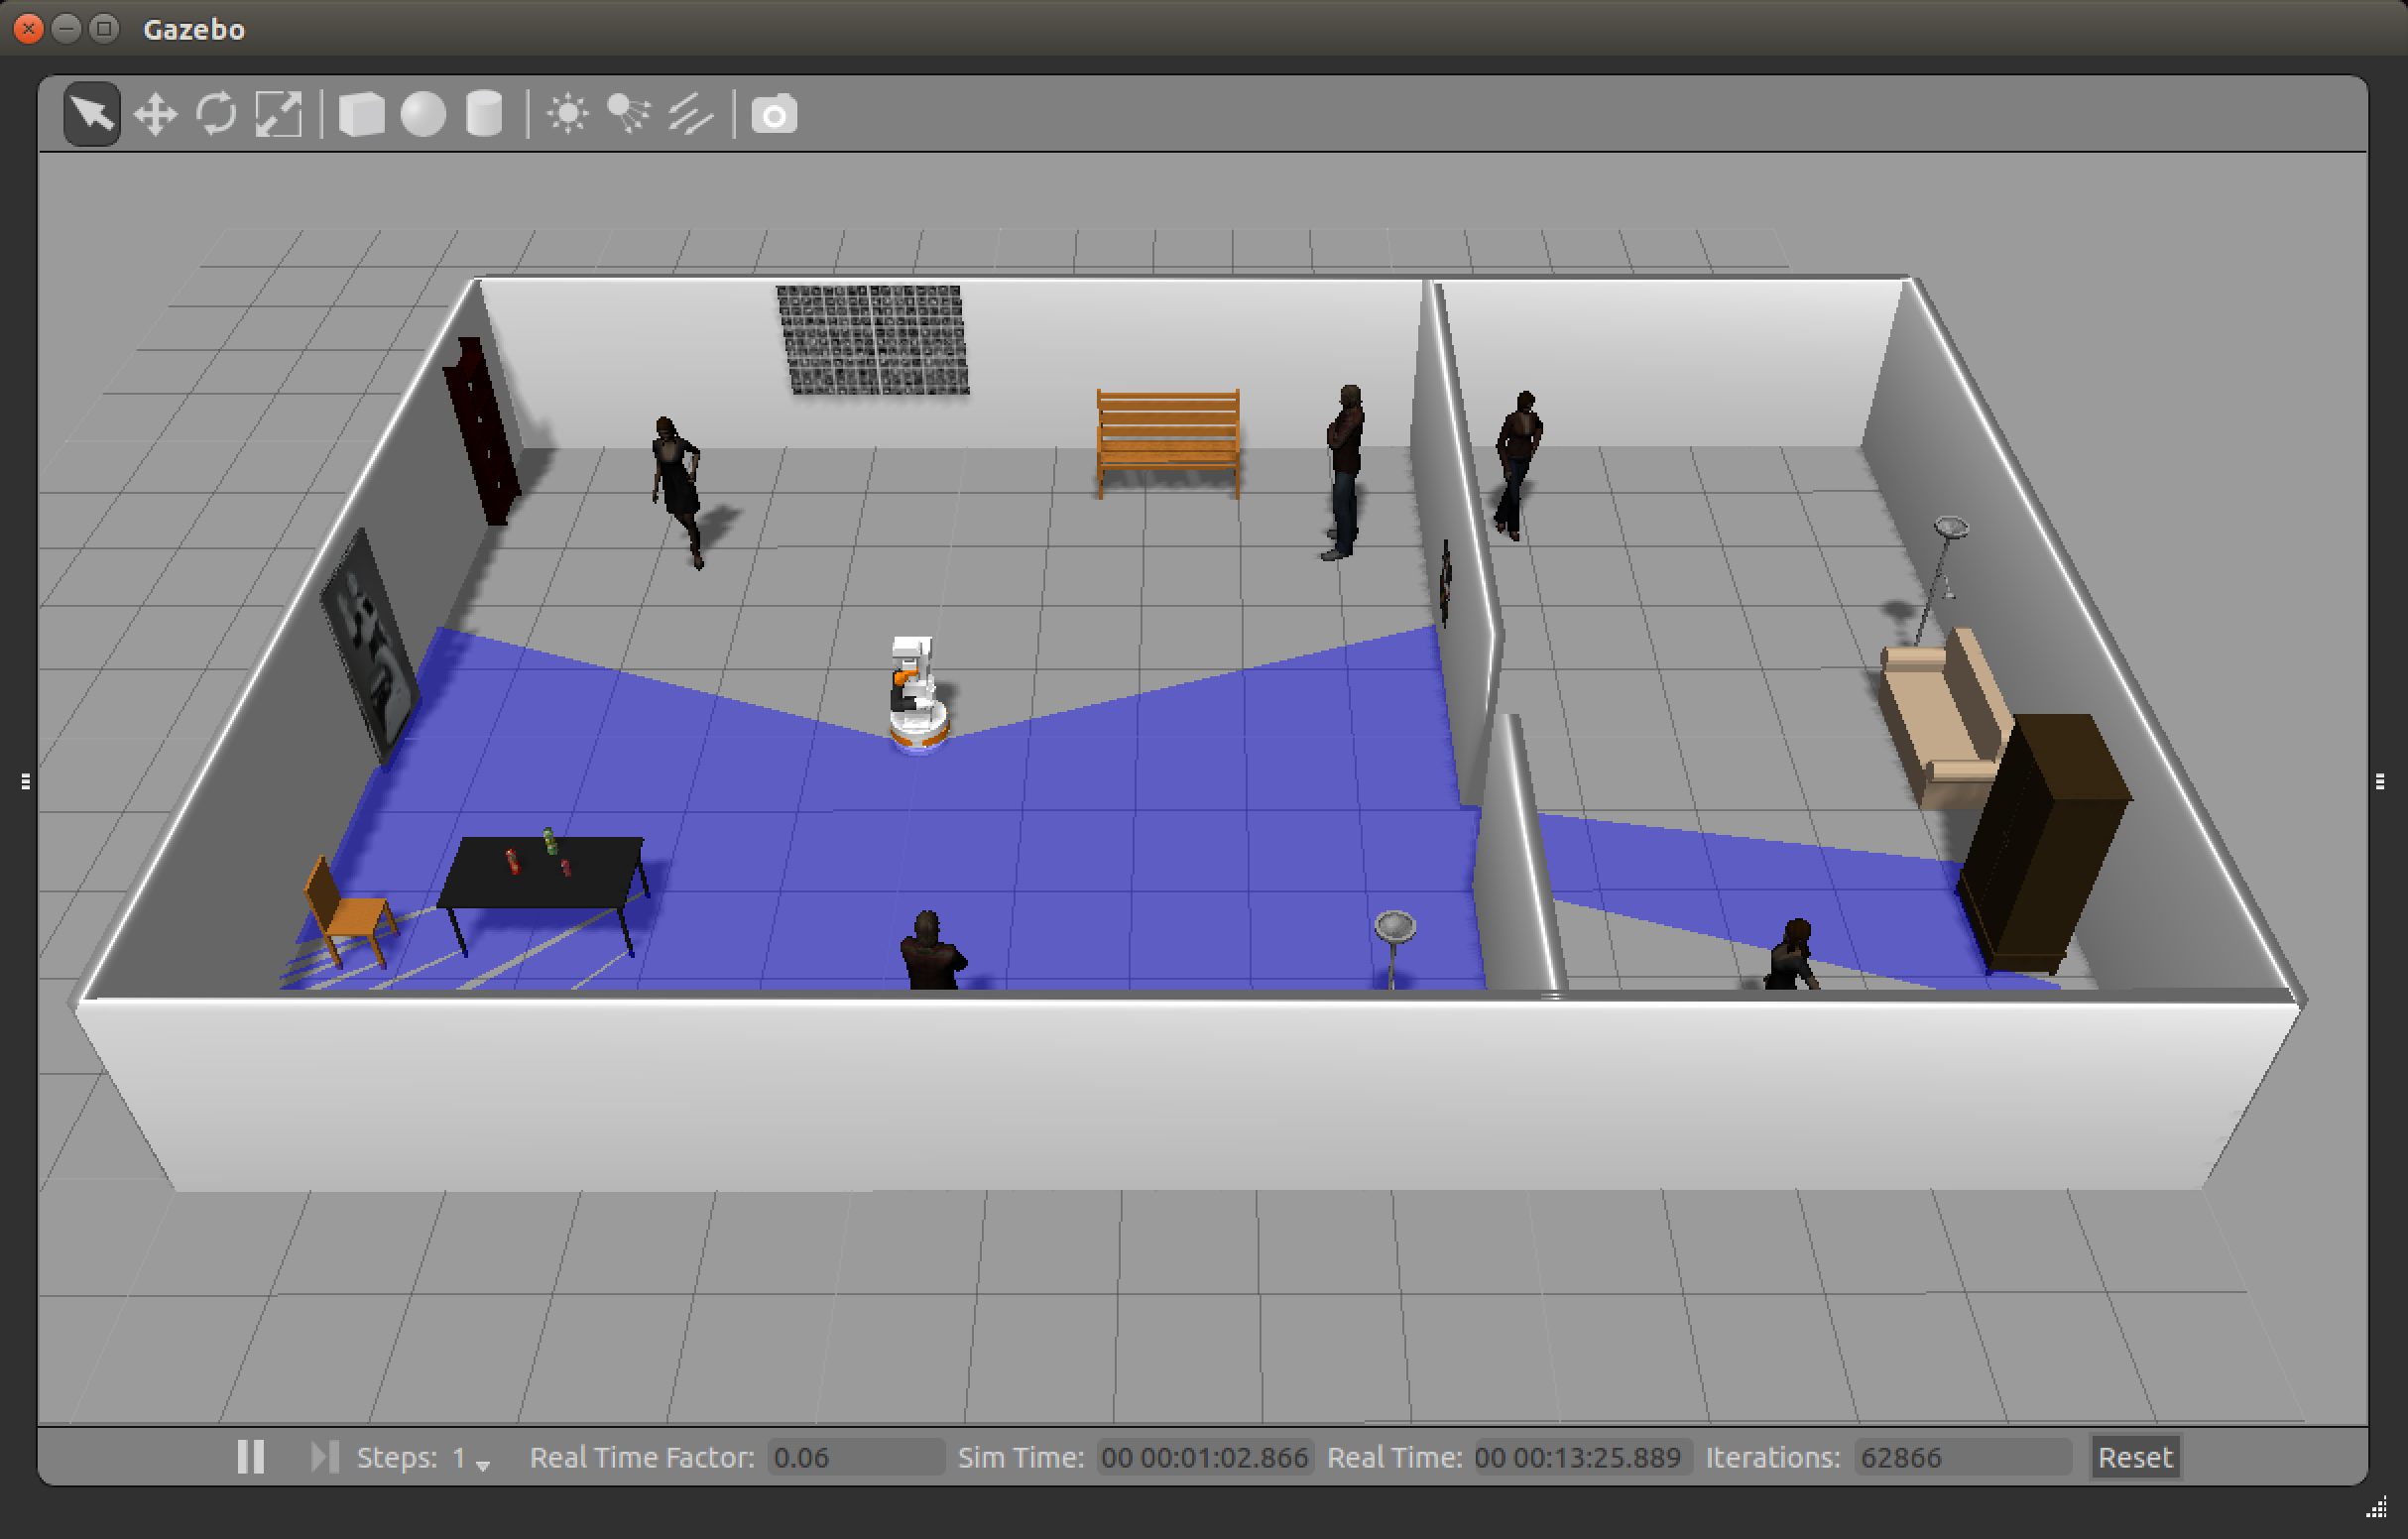
\includegraphics[width=11cm]{images/chapter2_gazebo_screenshot.png}
\end{center}
\caption{Gazebo Simulator (Office Environment).}
\label{fig:gazebo_screenshot}
\end{figure}

\section{RVIZ}

RVIZ is a 3D visualisation tool that provides information about what the robot is seeing, thinking and doing \cite{website:RVIZ}. Developing robotics application is by itself difficult, but without exactly knowing what the robot thinks is going on in the real world, it rises the level of complexity, as trying to debug only via numerical data is rather complicated especially at higher number of dimensions, which is common in the robotics field \cite{website:RVIZ}. 

Other important features that RVIZ offers via its modules are point cloud visualisation, laser-scan readings, coordinate frames as well as topological maps, obstacles data and current path visualisation when using the ROS navigation stack, making of RVIZ a powerful tool for this project and generally for the development of robot capabilities and research \cite{website:RVIZ}.

\begin{figure}[H]
\begin{center}
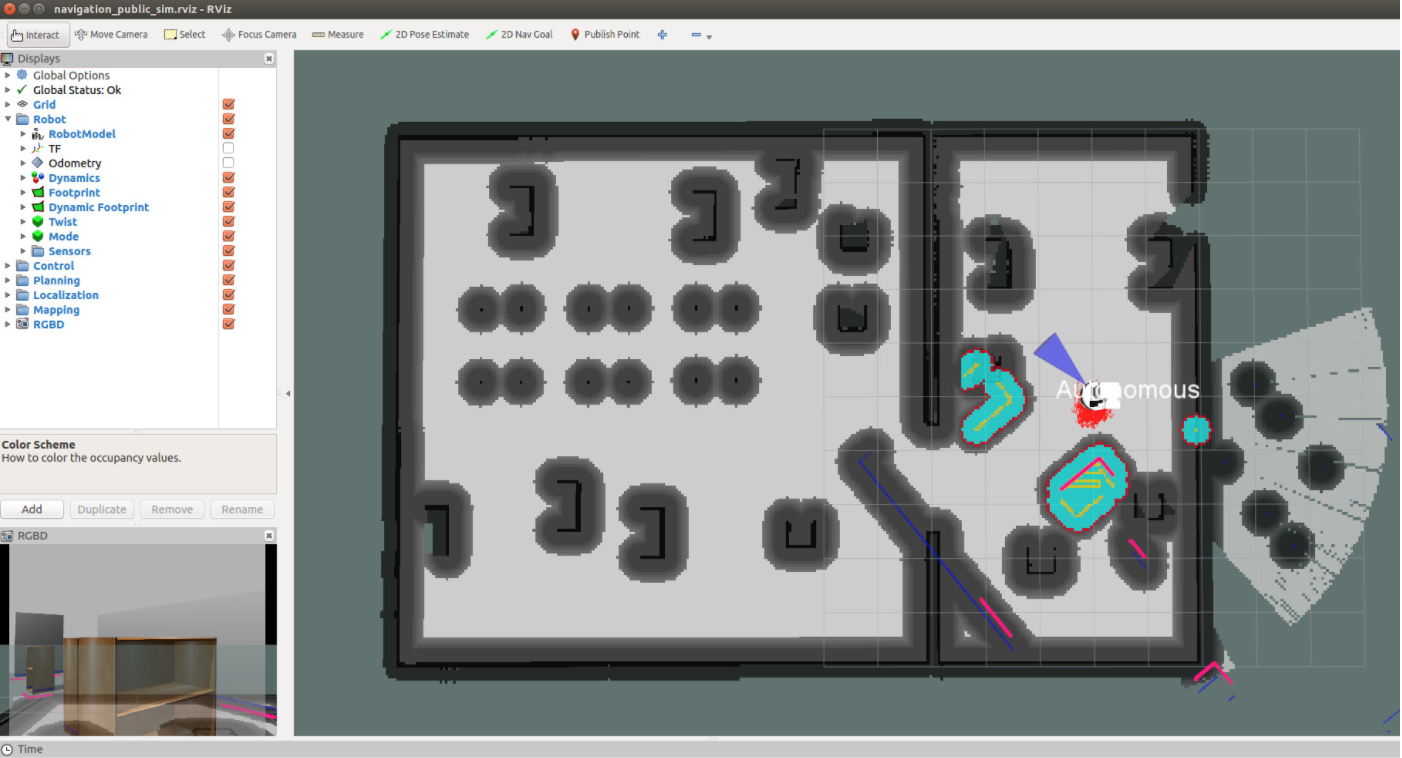
\includegraphics[width=11cm]{images/chapter2_rviz_screenshot.png}
\end{center}
\caption{RVIZ 3D visualisation.}
\label{fig:rviz_screenshot}
\end{figure}

\section{TIAGO}

TIAGO is a robot by PAL Robotics which was used throughout the project given its characteristics and sensory devices presented in the coming sections. 

In fact, it is a service robot designed to work in indoor environments \cite{website:TIAGo}, fitting the project's purpose of developing a ROS package for indoor human position estimation, whose output can be used to manoeuvre and interact around and with people.

Moreover, TIAGO's size and technical features make it an ideal platform for the project, combining many of the necessary sensors for the success of the end result. Including the RGB-D sensor, laser range finders and a differential-drive base to move around the environment.

\begin{figure}[H]
  \begin{center}
  	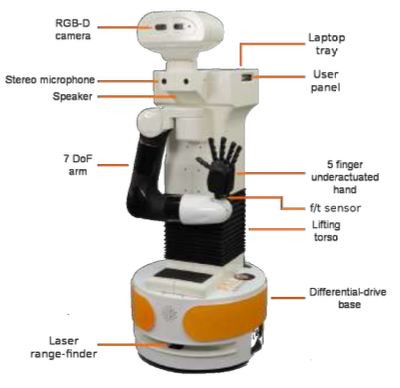
\includegraphics[width=6cm]{images/tiago_components.png}
  \end{center}
  \caption{TIAGO's components\protect\footnotemark.}
\end{figure}
\footnotetext{Picture Reference: \url{http://tiago.pal-robotics.com}}

\subsection{RGB-D}

The RGB-D sensor found on TIAGO, like other similar ones such as the Kinect, provides both colour information as well as the estimated depth for each pixel in the two dimensional colour image.

The depth per RGB pixel is provided by using a combination of the colour camera, an IR projector and an IR camera. The projector first shoots an infrared speckle pattern creating an irregular pattern of dots on the surface, due to the diffractive optical element of the projector \cite{paper:RGB-D}. The pattern is then captured by the IR camera, which compares the projected infrared pattern part-by-part to reference patterns stored in the device \cite{paper:RGB-D}. Finally, via this pattern reference the depth is computed using triangulation \cite{paper:RGB-D}. The Point-Cloud, a three dimensional space collection of points merging both RGB and depth information, is obtained by correlating the computed depths to a calibrated RGB camera with a known registration \cite{paper:RGB-D}.

TIAGO comes with an RGB-D camera integrated. More precisely, an Astra model with a minimum and maximum sensory range of respectively 0.6m and 8m.

\subsection{Lasers}

Laser range-finders is another important sensory device to have at disposal for this project, whose technological foundation is based on beam reflection and the time of flight.

Lasers send a pulse of light to a target and measure the time it takes for the reflection to come back \cite{website:lasers}. Therefore, by knowing the speed at which the beam travels (speed of light), and the time it takes for the pulse of light to be emitted and come back, the distance is easily computable using the velocity equation.

TIAGO comes with an integrated laser-range finder with a range of 0.05-25m and a 180\textdegree{} field of view. The frequency of the signal is of 15Hz.

\section{Person Detection}

Given the final aim of developing a ROS package able to estimate people's position, a person detection module able to detect humans in the available RGB sensory data is of critical importance.

Person detection is a popular and challenging task in computer vision. In fact, people have different features and can adopt diverse body poses. To complete such task, two viable solutions were identified.

The first approach consists in uses a combination of image gradients and the SVM machine learning model to classify whether people are present in the image. The second approach makes use of deep neural networks and their great accuracy.

The two solutions will be considered in this chapter only from a theoretical and algorithmic point of view, thereby highlighting the mechanics of both models.

\subsection{HOG (Histogram of Oriented Gradients)}

\subsubsection{Method Overview}

\begin{figure}[!htbp]
\begin{center}
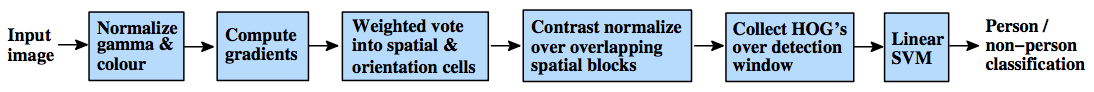
\includegraphics[width=\linewidth]{images/hog_chain.png}
\end{center}
\caption{HOG classification chain \cite{paper:dalal2005histograms}}
\label{fig:hog_chain}
\end{figure}

The method, whose feature extraction chain is shown in \ref{fig:hog_chain}, carries its evaluation on well-normalised local histograms of image gradient orientations in a dense grid \cite{paper:dalal2005histograms}. The idea behind the method is that object appearance and shape is most of the times characterised by the distribution of the local intensities of the gradients \cite{paper:dalal2005histograms}

After the normalisation process of the input, the image window is divided into small spatial regions called cells, where in each cell a local 1D histogram of gradient directions is computed by the sliding window technique \cite{paper:dalal2005histograms}, a process known as \textbf{spatial binning}. To improve light and shadowing invariance, local contrast-normalisation is also applied \cite{paper:dalal2005histograms}. The obtained HOG descriptors are then fed to a conventional SVM machine learning model resulting in the final human detection chain shown above \cite{paper:dalal2005histograms}.

The histogram based representation does offer some advantages. Mainly, it is robust to geometric and photometric transformations. Moreover possible translations or rotations do make little difference if these are smaller than the orientation bin size \cite{paper:dalal2005histograms}.

\subsubsection{Dataset}

The descriptor was tested on the MIT pedestrian database containing 509 training instances and 200 testing ones, plus the added mirror reflections \cite{paper:dalal2005histograms}. The best detector received a perfect detection result on the MIT dataset. A more challenging one was therefore created, where instances are still standing, but do appear on a variety of orientations and backgrounds. The model performed well once again, outperforming other models like Haar Wavelets \cite{oren1997pedestrian} and PAC-SIFT \cite{zhang2012adaptive} \cite{paper:dalal2005histograms}.

\begin{figure}[!htbp]
  \begin{center}
  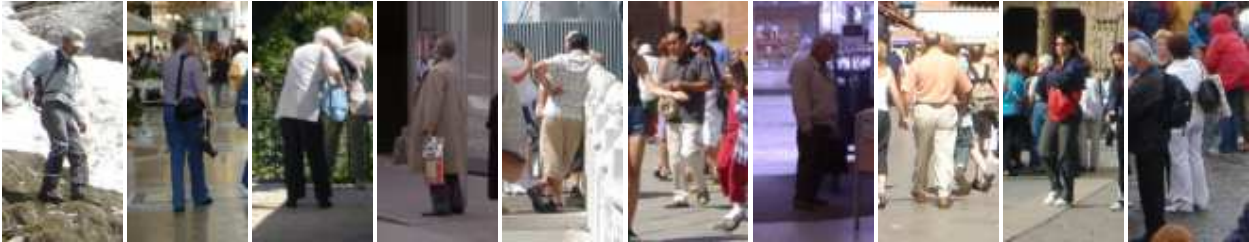
\includegraphics[width=\linewidth]{images/chapter6_mit_database.png}
  \end{center}
  \caption{MIT dataset sample images \cite{paper:dalal2005histograms}.}
  \label{fig:mit_dataset}
\end{figure}

\subsubsection{Implementation \& Performance Study}

The following subsection treats some of the details in the implementation of the HOG algorithm, as well as the effects in its performance when changing values related to:

\begin{itemize}
	\item Gamma/Colour Normalisation
	\item Gradient Computation
    \item Spatial/Orientation Binning
\end{itemize}

\subsubsection{Gamma/Colour Normalisation}

Several input pixel representations where evaluated, including grayscale, RGB and LAB colour spaces with gamma equalisation. However, these normalisations proved not to be effective on the ultimate results of the method \cite{paper:dalal2005histograms}.

\subsubsection{Gradient Computation}

The detector performance is really sensitive to the way in which gradients are computed \cite{paper:dalal2005histograms}. Several approaches were tested, including the Gaussian smoothing with different smoothing scales followed by 1D point derivatives. 3x3 Sobel masks were also used. However, the simplest approach gave the best result, which consisted in a 1D mask with a zero gamma correction \cite{paper:dalal2005histograms}. For colour images the gradients were computed separately for each colour channel \cite{paper:dalal2005histograms}.

\subsubsection{Spatial/Orientation Binning}

Each pixel calculates the weighted vote for an edge orientation histogram channel based on the orientation of the gradient element \cite{paper:dalal2005histograms}. These votes are then accumulated into orientation bins over the cell regions, where these can either be rectangular or radial and with 180\textdegree{} or 360\textdegree{} degree spacing. The vote is a function of the gradient magnitude itself, its square or its square root. However, in practice using the magnitude itself gives the best results \cite{paper:dalal2005histograms}.

Performance-wise, keeping the spatial binning coarse does not affect the performance, while increasing the number of orientation bins improves it up to 9 bins, after which no improvement is found \cite{paper:dalal2005histograms}.

\subsection{Deep Learning}

Deep learning is a subset of machine learning which has became a popular approach to solve computer vision problems since AlexNet in 2012 managed to improve object-detection accuracy using deep neural networks. Increased computational power and availability of large training data are two other important factors in the increased popularity of this approach.

Yann Lacun, Yoshua Benjo and Geoffrey Hinton defined deep learning as a computational model composed of multiple processing layers, able to learn the representation of data with multiple levels of abstraction \cite{paper:lecun2015deep}. Such methods have drastically improved the state-of-the-art in tasks like speech recognition, object recognition and object detection, by iteratively discovering large data sets' structure using the backpropagation algorithm, which helps the neural network update its parameters \cite{paper:lecun2015deep}.

Three deep-learning models were identified which are able to perform object detection at a high level of accuracy:

\begin{enumerate}
  \item YOLO\footnote{You Only Look Once} \cite{paper:YOLO}
  \item Faster R-CNN \cite{paper:FRCNN}
  \item SSD\footnote{Single Shot Multibox Detector} \cite{paper:SSD}
\end{enumerate}

Given the subtle differences in the classification accuracy of the above neural networks, the SSD model was chosen for its computational efficiency and therefore its speed of detection over the other two. The MobileNet version of the SSD model was used in particular for its added computational optimisation, which is especially important for power constrained devices, as well as its ease to be embedded within a system.

\subsubsection{SSD Overview}

The SSD model is a single deep neural network able to detect various objects in a scene by discretising the output space with bounding boxes over different aspect ratios and scales per feature map \cite{paper:SSD}, and where feature maps identify the various activation layers. During the feed-forward prediction process, scores are generated for the presence of each object category in each bounding box, along with an adjustment to the bounding boxes to better match the object shape \cite{paper:SSD}. The network also combines various feature maps predictions with different resolutions to handle objects of various sizes \cite{paper:SSD}. Moreover, the SSD's classification process is simpler than other state-of-the-art models such as Faster R-CNN \cite{paper:FRCNN}, as the former does not require proposal regions and subsequent pixel re-sampling stages, thereby encapsulating all required computations in a single network making the model easy to train and straightforward to integrate into systems that require a detection component \cite{paper:SSD}.

\subsubsection{SSD Architecture}

Current state-of-the-art object detection models are variances of the same detection process, which includes the following steps \cite{paper:SSD}:

\begin{enumerate}
  \item Hypothesise bounding boxes
  \item Pixel or features re-sampling
  \item Classification
\end{enumerate}

Although the above pipeline has proved to obtain great accuracy results, it has the major drawback of being too computationally expensive for real-time applications \cite{paper:SSD}. The SSD model improves upon Faster R-CNN \cite{paper:FRCNN} and YOLO \cite{paper:YOLO} by removing the need for bounding box proposals and the re-sampling processes, while still retaining the same accuracy performance using separate small convolutional filters applied at different aspect ratios \cite{paper:SSD}. These  filters are also applied to multiple feature maps from the later stages of the network in order to perform detection at multiple scales \cite{paper:SSD}.

\begin{figure}[!htbp]
\begin{center}
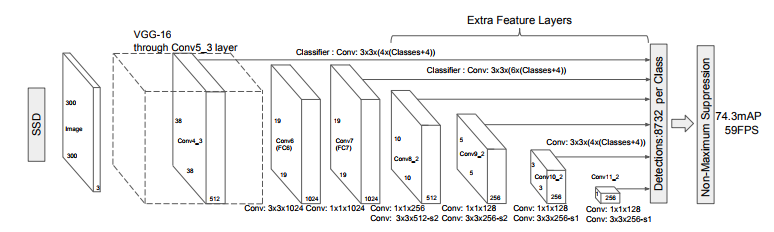
\includegraphics[width=\linewidth]{images/ssd_architecture.png}
\end{center}
\caption{SSD Model \cite{paper:SSD}.}
\label{fig:sshModel}
\end{figure}

The SSD architecture shown in \ref{fig:sshModel} presents a standard base network (VGG-16) used for high quality image classification, upon which auxiliary layers are added to produce detections with the following key features \cite{paper:SSD}:

\begin{enumerate}
  \item Multi-scale feature maps
  \item Convolutional predictors
  \item Default boxes and aspect ratios
\end{enumerate}

\textbf{Multi-scale feature maps}

Convolutional feature layers are added at the end of the truncated base network with the aim of progressively decreasing the input image size, therefore allowing for detections at multiple aspect ratios \cite{paper:SSD}. Different convolutional filters are used for each feature layer \cite{paper:SSD}.

\textbf{Convolutional predictors}

Each added feature layer on top of the base network can produce a fixed set of detection predictions using the previously mentioned convolutional filters \cite{paper:SSD}. Generally speaking, a feature layer of size m x n with p channels requires a 3 x 3 x p kernel to produce either a score for a category, or a bounding box offset relative to a default box position for each feature map location \cite{paper:SSD}.

\textbf{Default boxes and aspect ratios}

A set of default bounding boxes is associated for each feature map cell for multiple feature maps at the top of the network (straight after the base network truncation) \cite{paper:SSD}. The relative offsets to the default box shapes (i.e. the ground truths), as well as the per-class scores indicating the presence of a class instance in each of those boxes is computed at each activation layer (i.e. feature map) \cite{paper:SSD}. Specifically, for each box out of k, the \textit{c} class score is computed as well as the four offsets. In fact, for each discretised point in the original image, four bounding boxes are drawn with different aspect ratios \cite{paper:SSD}, as shown in the images below.

\begin{figure}[!htbp]
\begin{center}
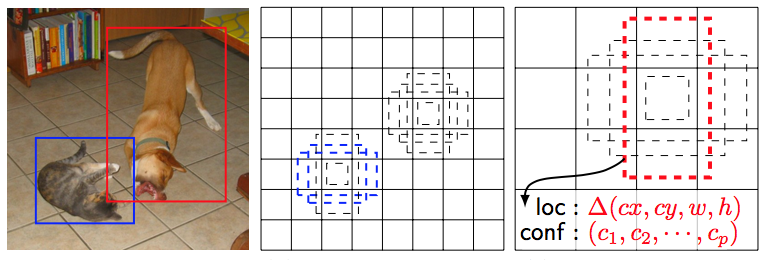
\includegraphics[width=\linewidth]{images/gt_boxes.png}
\end{center}
\caption{Ground truth, feature maps, offset computation \cite{paper:SSD}.}
\label{fig:ssdGT}
\end{figure}

\subsubsection{MobileNets}

MobileNet provides an efficient network architecture in order to build small and low latency models that can be easily embedded in vision applications running on limited devices \cite{paper:MobileNets}. In fact, although the SSD model is relatively computationally lightweight compared to other state-of-the-art models, it is still not enough to carry real-time detections on computationally limited platforms.

The MobileNet structure is built on top of depthwise separable convolutions, except for the first layer which is a full convolutional layer \cite{paper:MobileNets}. This approach enables to further discover other possible network topologies for a better performance overall. The MobileNet architecture is presented below:

\begin{figure}[H]
\begin{center}
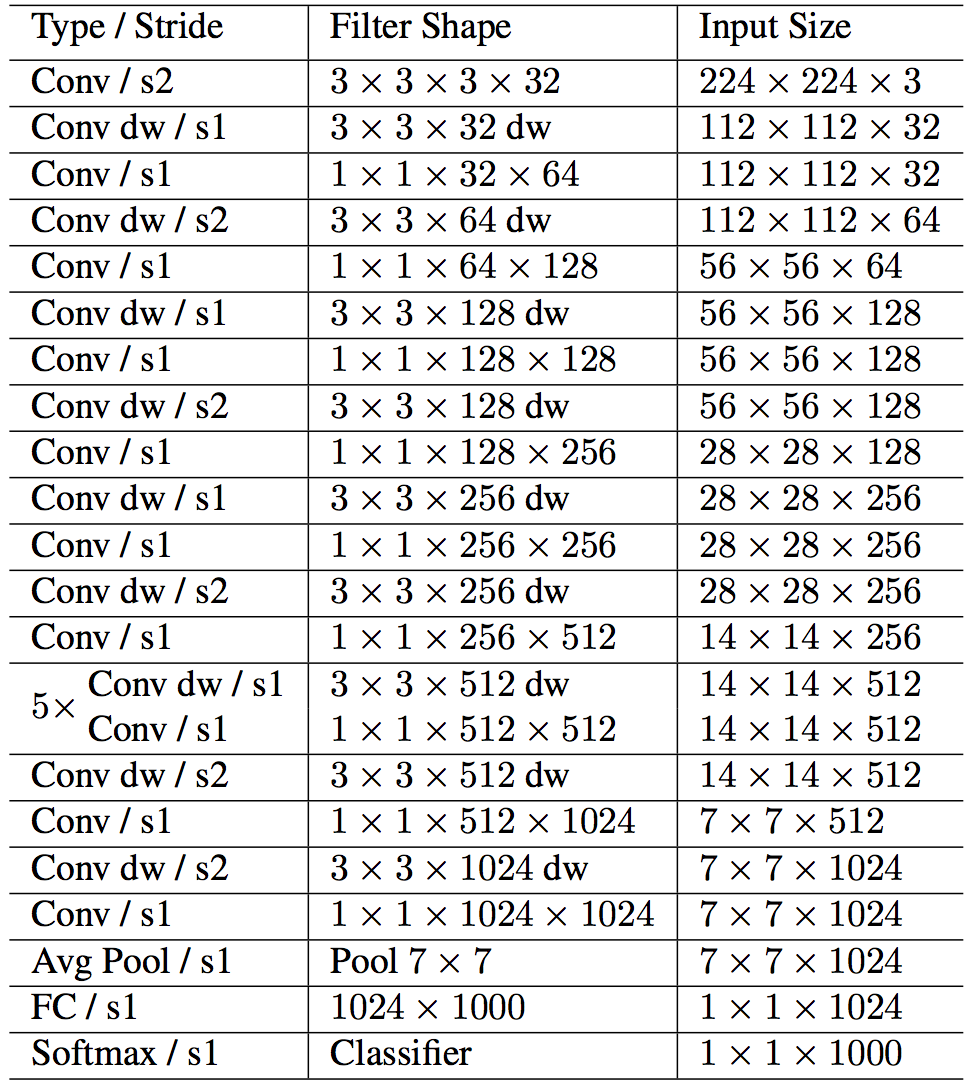
\includegraphics[width=7cm,height=9cm,keepaspectratio]{images/mobileNet_structure.png}
\end{center}
\caption{MobileNet Architecture \cite{paper:MobileNets}.}
\end{figure}

Each layer component in the network is followed by a batch-normalisation and a rectified linear unit, with the sole exception of the final layer which feeds directly into the softmax layer for the classification \cite{paper:MobileNets}. Furthermore, the down sampling is handled with strided convolutions in the depthwise convolutions as well as in the first layer. A final average pooling does reduce the overall spatial resolution before the fully connected layer, with a total of 28 layers \cite{paper:MobileNets}.

\begin{figure}[!htbp]
\begin{center}
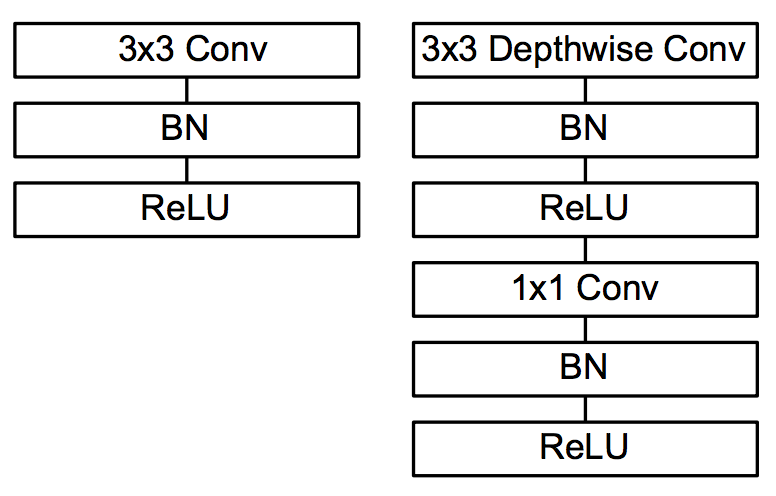
\includegraphics[width=7cm,height=9cm,keepaspectratio]{images/mobileNet_contrast.png}
\end{center}
\caption{Standard convolutional (left), Depthwise Separable convolutions (right) \cite{paper:MobileNets}.}
\end{figure}

\subsubsection{Depthwise Separable Convolution}

The depthwise separable convolution is a factorised convolution which factorises a standard convolution into a depthwise one and a 1x1 convolution called pointwise convolution \cite{paper:MobileNets}.

The main difference between a usual convolution and the depthwise convolution is that the former applies both a filtering and a combination procedure to the set of inputs into a new set of outputs in a single step \cite{paper:MobileNets}. The latter, however, splits the procedure into two separate layers. This separation drastically reduces the computation and model size. The figure below shows a standard convolution (a), a depthwise convolution (b) and a 1x1 pointwise convolution (c).

\begin{figure}[H]
\begin{center}
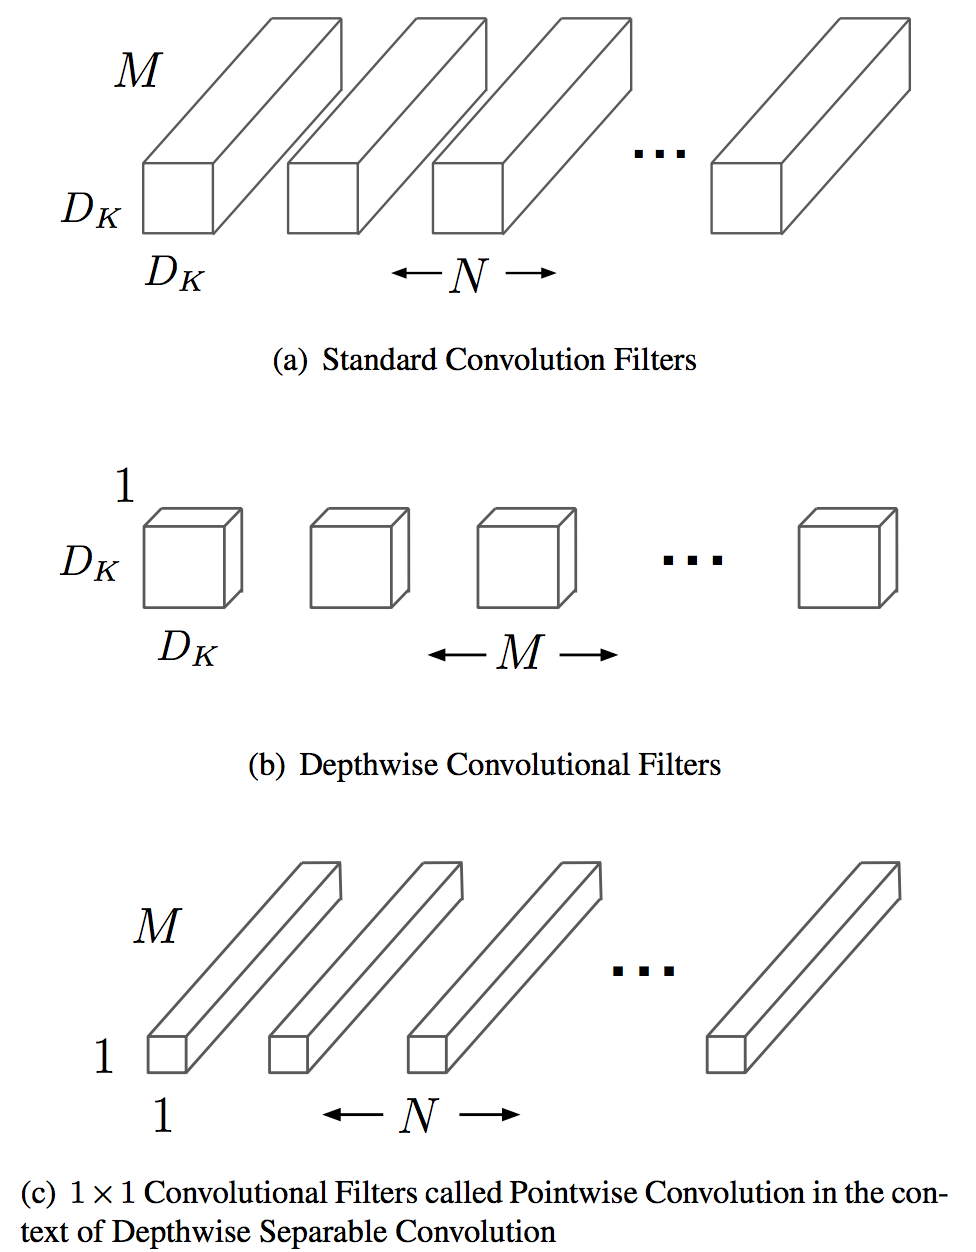
\includegraphics[width=5cm,height=7cm,keepaspectratio]{images/convolutions.png}
\end{center}
\caption{Depthwise convolution transformation \cite{paper:MobileNets}.}
\end{figure}

\subsubsection{Width and Resolution Multipliers}

The basic MobileNet architecture already offers a better efficiency by being smaller and with a lower latency than usual networks. Nonetheless, many times specific applications require a model which is even smaller and less computationally expensive. The width and resolution hyper-parameters serve exactly this.

The width multiplier defined with the greek letter \textit{alpha} has the role to thin the network layers uniformly \cite{paper:MobileNets}. Usual values for \textit{alpha} are between 0 and 1, with 1 being the model baseline for MobileNet. Usually, the smaller the parameter the smaller the model will be, and hence the less accurate \cite{paper:MobileNets}.

The second hyper-parameter to reduce the computational cost of a general neural network is the resolution multiplier defined with the greek letter \textit{p} \cite{paper:MobileNets}. The parameter is directly applied to the input image, and the internal representation of every layer is subsequently reduced by the same multiplier \cite{paper:MobileNets}. Typical values for \textit{p} are between 0 and 1, with 1 being the MobileNet baseline \cite{paper:MobileNets}.

\begin{figure}[!htbp]
\begin{center}
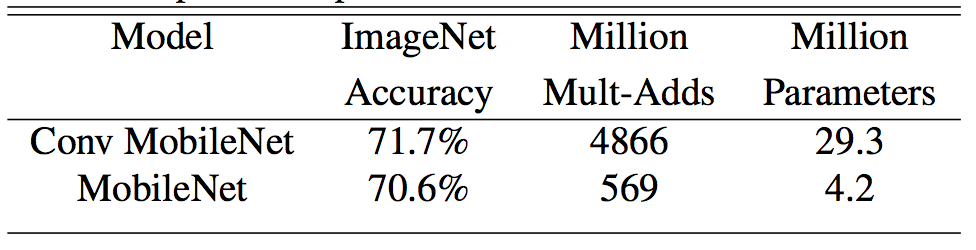
\includegraphics[width=10cm,height=10cm,keepaspectratio]{images/mobileNet_table.png}
\end{center}
\caption{Full vs Depthwise convolutions performance comparison \cite{paper:MobileNets}.}
\end{figure}

\section{Distance Estimation}

To be able to estimate the 3D position of a person, the only RGB detection is not enough. The distance from the robot to the person is also required. Hence three approaches were identified as a possible solution to the task.

The first approach consists in using the RGB-D sensor which comes integrated on TIAGO, presented in Chapter1. The second approach uses the Triangulation technique, a common computer vision algorithm to obtain depth from two or more viewpoints. Finally, the usage of the on-board laser-scan sensor and its long-range is also considered so as to detect people's leg, thereby finding their distance from the robot.

\subsection{RGB-D Mapping}

The RGB-D camera integrated in TIAGO offers a variety of topics from which valuable sensory data can be retrieved. In particular the depth map and possibly the point cloud are the data of interest, as these respectively offer the distance in metres for every RGB pixel, which is exactly what is required.

Therefore, by using the existing knowledge of where the bounding box outlining the person's figure is in the two dimensional RGB frame, a known point on the person  can be mapped to the point cloud or depth-image, ultimately finding the corresponding depth of the pixel.

However, sensors are not perfect, especially in the real world where noise is present, therefore such a solution could be integrated together with one of the another two methods for a better distance estimation.

\subsection{Triangulation}

The problem consists in finding the position of a point in space, given its location in two images taken with different cameras and know calibration and pose \cite{hartley1997triangulation}. The process requires to find the intersection of the two known rays in space, which is trivial when noise is absent, however, this is most likely not the case and consequently the rays might never intersect \cite{hartley1997triangulation}. Therefore, it is necessary to find the best possible point, consequently reducing the problem to an optimisation one \cite{hartley1997triangulation}.

The paper presents a solution to the problem by assuming a Gaussian noise model for perturbation of the image coordinates, and by formulating it as a least-squares minimisation problem.

\subsubsection{Formulation}

Supposing a point x is present in at least two images and that the two camera matrices, P and P' which define the extrinsic and intrinsic camera information are known, u and u' are identified as the projections of such point x in the two images \cite{hartley1997triangulation}, and whose intersection is the target.

A commonly suggested method is to choose the midpoint of the common perpendicular to the two rays \cite{hartley1997triangulation}. However, such way would not give an optimal result due to the various approximations made \cite{hartley1997triangulation}. Hence, a new formulation is made that relies on the concepts of epipolar correspondence and the fundamental matrix \cite{hartley1997triangulation}. The algorithm presented, moreover, is claimed to be moderate in computation requirements due to its non-iterative nature and calculus based approach \cite{hartley1997triangulation}.

\subsubsection{Minimisation Criterion}

The method sets some criteria with regards to the good result of the triangulation process. These are the following:

\begin{enumerate}
  \item The camera matrices and the fundamental matrix \textbf{F} are known
  \item The projection points satisfy the fundamental matrix constraint
  \item The image features noise model is a Gaussian
\end{enumerate}

Upon these assumptions the projection points u and u' that are seeked are the ones that minimises the following function \cite{hartley1997triangulation}:

\[d(u, u')^2 + d(u', u)^2\]

where d(*, *) represents the Euclidean distance subject to the epipolar constraint \cite{hartley1997triangulation}:

\[u'Fu = 0\]

Assuming a Gaussian error distribution, the points u and u' are the value for the true image point correspondence, and once these are computed through the resolution of the epipolar constraint equation, the point x, holding the distance value,  may be found by using any triangulation technique such as Linear Triangulation \cite{hartley1997triangulation}.

\subsubsection{Linear Triangulation}

Supposing:

\[u = Px\]

the left hand-side can be written in homogeneous coordinates \cite{hartley1997triangulation}:

\[u = w(u, v, 1)^T\]

where (u,v) are the observed point coordinates and w is the unknown scale factor \cite{hartley1997triangulation}. By denoting every ith row of the matrix P, the equation \textbf{u = Px} may be written as \cite{hartley1997triangulation}:

\[wu = p1^Tx, wv = p2^Tx, w = p3^Tx\]

Which upon substituting the w using the third of the equations, the following is obtained \cite{hartley1997triangulation}:

\[up3^T = p1^Tx\]
\[vp3^T = p2^Tx\]

The set of linear equations can be written in the form of \textbf{Ax = 0}, finally solving for x \cite{hartley1997triangulation}. Several algorithms can be used to solve the linear system of equations for x, including the Linear-Eigen method or an iterative one such as the Gauss-Seidel algorithm \cite{hartley1997triangulation}.

\subsection{Leg Detection}

RGB-D sensory data are not the only available choice to compute the required distance. In fact, TIAGO is incorporated with both sonar and laser-scan sensors. Due to the physical properties behind the two that make laser-scan more accurate for the project's purpose, and faster because the speed of light is higher then the speed of sound, as well as the current availability of external ROS packages to find legs pattern in laser's data, the latter sensor is chosen over the former.

\subsubsection{Introduction}

\begin{figure}[H]
\begin{center}
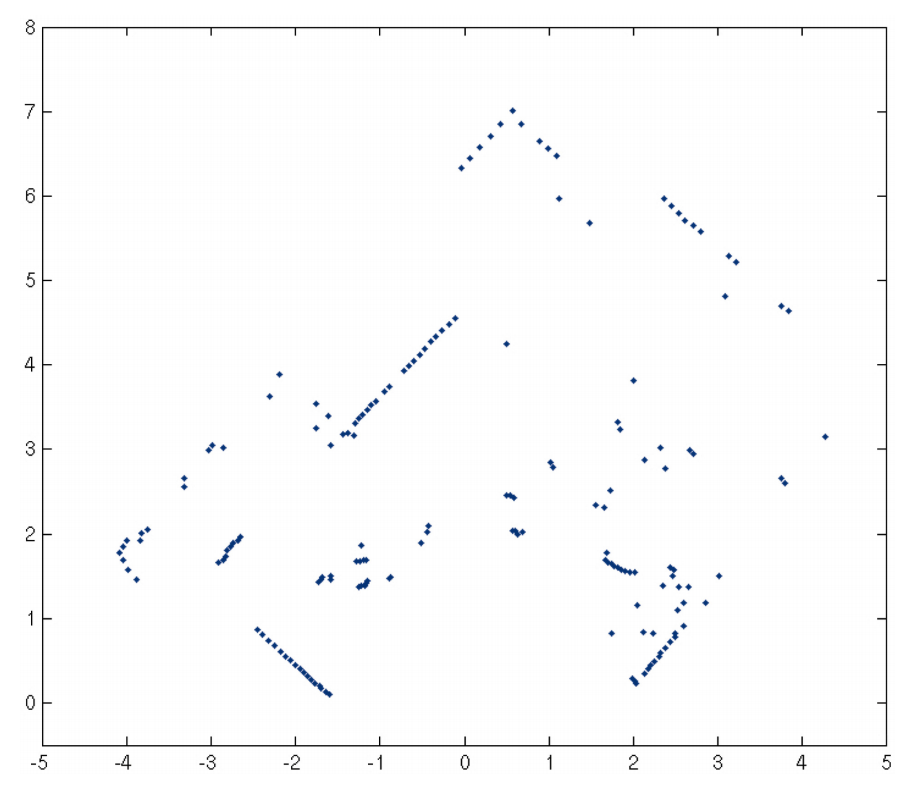
\includegraphics[width=.4\linewidth]{images/laser-data.png}
\end{center}
\caption{Laser data in a typical office environment \cite{arras2007using}.}
\label{figːlaser_data}
\end{figure}

The problem addressed regards detecting people in two dimensional range scans, using supervised machine learning techniques to create a classifier that facilitates such detection \cite{arras2007using}. However, laser data contain little to no information about people, as they typically consist of plain two-dimensional range information \cite{arras2007using}.

Figure \ref{figːlaser_data} shows an example of such data in a cluttered office environment, where several people walked through during the data recording. This is to show how difficult it is to recognise leg patterns by merely looking at the data \cite{arras2007using}. In fact, even humans would be in difficulty performing such a task.

However, laser measurements that correspond to human legs do have certain geometrical properties \cite{arras2007using}. Size, circularity, convexity and compactness are some of these, as shown in \ref{figːleg_scans} \cite{arras2007using}. Therefore, by determining a set of numerical features that define these geometrical properties, a supervised machine learning model can then be used to create a people detector \cite{arras2007using}, and from which the distance can be retrieved.

Other approaches for person detection in range scans where also studied before. One of the most popular one is to extract legs by detecting moving blobs in the range image \cite{fod2002laser}, \cite{kleinehagenbrock2002person}, \cite{scheutz2004fast}, \cite{schulz2003people}, \cite{arras2007using}. This motion range feature type of detection requires a scan matching procedure so as to align the two subsequent scan and perform the subtraction, ultimately incurring in added computational costs \cite{arras2007using}. Moreover, the detection would only be limited to people in motion. Hence the decision to pursue a geometry features based detection.

\begin{figure}[H]
\begin{center}
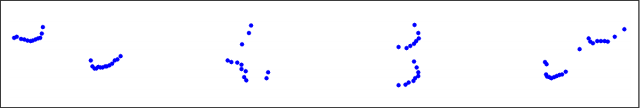
\includegraphics[width=.4\linewidth]{images/leg_scans.png}
\end{center}
\caption{Typical range readings from legs of people \cite{arras2007using}.}
\label{figːleg_scans}
\end{figure}


\subsubsection{Boosting}

Boosting is a general method for creating an accurate classifier by combining a set of weak classifiers \cite{arras2007using}. The AdaBoost algorithm introduced by Freud and Schapire \cite{schapire1999improved} is used for the classification process \cite{arras2007using}. More precisely, the input to the AdaBoost algorithm used is a set of labelled training data, where each instance is assigned to a weak classifier using a weight distribution over the input \cite{arras2007using}, which ultimately will have a small classification error corrected iteratively by modifying the weight distribution of the examples \cite{arras2007using}. The final strong classifier will be a weighted majority vote of the T best weak classifiers \cite{arras2007using}.

\subsubsection{Segmentation \& Features}

The robot is already equipped with a range sensor that delivers observations as a set of returned beams, where each one of these is in the form of a tuple containing both the angle of the beam relative to the robot, and the length of the beam itself \cite{arras2007using}, which is exactly what TIAGO's hardware interface provides. Furthermore, the set of beams returned is split on smaller subsets grouped together based on a distance metric. Such that if two adjacent beams are farther away than a certain threshold distance, a new subset is initialised. The segmentations can therefore be readily processed by the subsequent learning step \cite{arras2007using}. Premebida and Nunes present a more adaptive segmentation technique which comes at the cost of added complexity in \cite{premebida2005segmentation}.

Fourteen different features were chosen for the binary classification, including mean curvature, mean average deviation from median, circularity and linearity among others \cite{arras2007using}. Each feature \textit{f} is then defined as function f:S -> R that takes a segment instance and returns a real value. The collection of the feature's values constitutes a profile for the segment which is classified by the AdaBoost algorithm \cite{arras2007using}. Figure \ref{fig:features} shows a typical segment profiling.

\begin{figure}[!htbp]
\begin{center}
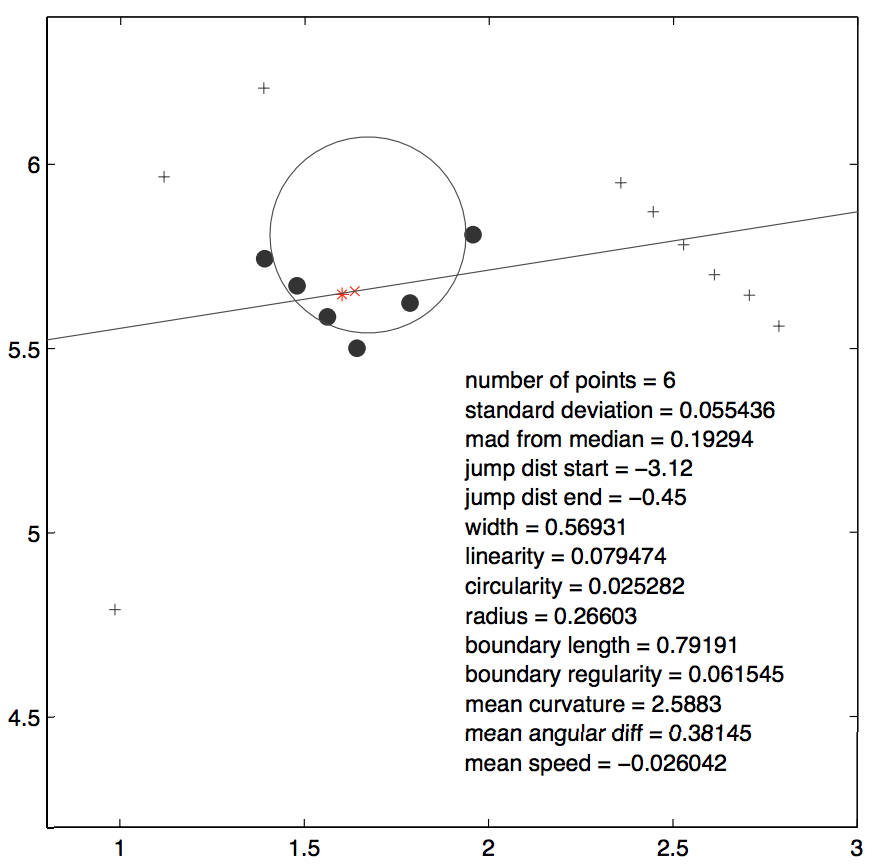
\includegraphics[width=.4\linewidth]{images/segment_profile.png}
\end{center}
\caption{Segment profile \cite{arras2007using}.}
\label{fig:features}
\end{figure}

\subsubsection{Results}

Although the algorithm still suffers from data association problems due to the complexity of the task, especially when several people are standing close together, the results obtained from its testing in cluttered environments, such as corridors and offices, are encouraging with a detection rate of over 90\% \cite{arras2007using}.

\begin{figure}[!htbp]
\begin{center}
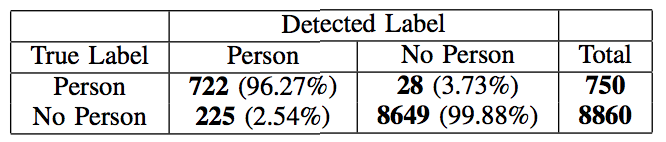
\includegraphics[width=.5\linewidth]{images/leg_cfm.png}
\end{center}
\caption{Confusion Matrices in office and corridor environments \cite{arras2007using}.}
\end{figure}